\documentclass{beamer}
%
% Choose how your presentation looks.
%
% For more themes, color themes and font themes, see:
% http://deic.uab.es/~iblanes/beamer_gallery/index_by_theme.html
%
\mode<presentation>
{
  \usetheme{default}      % or try Darmstadt, Madrid, Warsaw, ...
  \usecolortheme{beaver} % or try albatross, beaver, crane, ...
  \usefonttheme{structurebold}  % or try serif, structurebold, ...
  \setbeamertemplate{navigation symbols}{}
  \setbeamertemplate{caption}[numbered]
}

\usepackage[english]{babel}
\usepackage[utf8x]{inputenc}
\usepackage{hyperref}

%%%%%%%%%%%%%%%%%%%%%%%%%%%%%%%%%%%%%%%%%%%%%
% Slide 1
\title[Real-life systems]{Real-life systems}
\author{Manoj Gudi}
\institute{Ex-R.A. FOSSEE | CTO | Focus Analytics}
\date{6th February 2017}

\begin{document}
\begin{frame}
  \titlepage
\end{frame}

% Uncomment these lines for an automatically generated outline.
%\begin{frame}{Outline}
%  \tableofcontents
%\end{frame}

%%%%%%%%%%%%%%%%%%%%%%%%%%%%%%%%%%%%%%%%%%%%%%
%%%%%%%%%%%%%%%%%%%%%%%%%%%%%%%%%%%%%%%%%%%%%%
\section{Introduction}
%%%%%%%%%%%%%%%%%%%%%%%%%%%%%%%%%%%%%%%%%%%%%%
%%%%%%%%%%%%%%%%%%%%%%%%%%%%%%%%%%%%%%%%%%%%%%
% Slide 2
\begin{frame}{Content \& Scope}
\begin{itemize}
  \item Stateful system
  \item Observer Design Problem
  \item Approaches to solve this problem
  \item Examples using scilab
  \item How we use it to solve our problems
  \item \textbf{Not} rigorous and \textbf{barely} exhaustive
  \item Should be enough to get started to solve simple problems
\end{itemize}
\vskip 1cm
\end{frame}
%%%%%%%%%%%%%%%%%%%%%%%%%%%%%%%%%%%%%%%%%%%%%%
% Slide 2
\begin{frame}{Motivation..}

\begin{itemize}
  \item Estimation: \textit{a rough calculation of the value, number, quantity, or extent of something.}
  \item Humans estimate all the time
  \item Useful and practical estimations:
  \begin{itemize}
    \item Movement of cyclones while weather forecasting
    \item Value of a stock in equity market
    \item Predicting and correcting flight path by it's position
    \item Estimating length of this talk by number of slides
  \end{itemize}
\end{itemize}
\vskip 1cm
\end{frame}

%%%%%%%%%%%%%%%%%%%%%%%%%%%%%%%%%%%%%%%%%%%%%%%
% Slide 3
\begin{frame}{..Motivation}

\begin{itemize}
  \item Each estimation is prone to errors
  \begin{itemize}
    \item Difficult to track cyclone because of complex models
    \item Too much volatility in markets due to external factors
    \item Noisy data from sensors, susceptible to failure
    \item Speaker was a student not too long ago, knows how to hide no. of slides
  \end{itemize}
  \item Metrics of real-life systems are often difficult to measure and noisy
\end{itemize}
\vskip 1cm
\end{frame}

%%%%%%%%%%%%%%%%%%%%%%%%%%%%%%%%%%%%%%%%%%%%%%
% Slide 4
\begin{frame}{State..}

\begin{itemize}
  \item \textbf{State variable}: A state variable is one of the set of variables that are used to describe the mathematical "state" of a dynamical system.\textit{Wiki}
  \item Distance, velocity represent the state of a moving vehicular system.
  \item Current and Volt are state variables for a circuit.
  \item Set of possible values of state variables is \textit{State Space}.
  \item States are usually what we want to measure, but can\'t.
  \item Hence we resort to estimating/deducing state value by observing system behavior.
\end{itemize}
\vskip 1cm
\end{frame}

%%%%%%%%%%%%%%%%%%%%%%%%%%%%%%%%%%%%%%%%%%%%%%%
% Slide 5
\begin{frame}{..State}

\begin{itemize}
  \item States for examples from above slides
  \begin{itemize}
    \item Position of the eye of the cyclone
    \item Stock price of a company share in market
    \item Position of an airplane in sky
    \item Duration of talk
  \end{itemize}
  \item States can be continuous or discrete variables. The above ones are discrete.
  \item States is what we want to measure precisely, but most of the times we can't
\end{itemize}
\vskip 1cm
\end{frame}

%%%%%%%%%%%%%%%%%%%%%%%%%%%%%%%%%%%%%%%%%%%%%%%%
% Slide 6
\begin{frame}{State variables}

\begin{itemize}
  \item States for examples from above slides
  \begin{itemize}
    \item Position of the eye of the cyclone
    \item Stock price of a company share in market
    \item Position of an airplane in sky
    \item Duration of my talk
  \end{itemize}
  \item States can be continuous or discrete variables. The above ones are discrete.
  \item State is what we want to know, but most of the times we can't measure precisely
\end{itemize}
\vskip 1cm
\end{frame}
%%%%%%%%%%%%%%%%%%%%%%%%%%%%%%%%%%%%%%%%%%%%%
% Slide 7
\section{Observer Design Problem}
\begin{frame}{Observer Design Problem}

\begin{itemize}
  \item Basic problem is to determine/estimate internal states of a linear system
  \item System's output can be precisely measured
  \item Access to internal states of this system is assumed
  \item A change in internal state is directly reflected in system's outputs
  \item Can be modelled it as a black box where we have
  \begin{itemize}
    \item Sampled measurements
    \item A process model
    \item A measurement model
  \end{itemize}
\end{itemize}
\vskip 1cm
\end{frame}
%%%%%%%%%%%%%%%%%%%%%%%%%%%%%%%%%%%%%%%%%%%%%
% Slide 8
\section{Models}
\begin{frame}{Process Model}
\begin{itemize}
  \item Linear discrete time invariant process model \[ x_k = Ax_{k-1} + Bu_k + w_{k} \]
  \item \(x_k\) represents current state  \(x_{k-1}\) represents previous state
  \item A is state transition matrix and B is control input matrix \(u_k\) is control input
  \item \(w_{k}\) is Gaussian process noise (i.e. mean is 0)
  \item This equation gives insights how current state and input affects the future state
\end{itemize}
\vskip 1cm
\end{frame}
%%%%%%%%%%%%%%%%%%%%%%%%%%%%%%%%%%%%%%%%%%%%%
% Slide 9
\begin{frame}{Measurement Model}
\begin{itemize}
  \item \[ y_k = Hx_{k} + v_k \]
  \item \(y_k\) is the vector of measurement
  \item \(H_t\) is the transformation matrix that maps state vector parameters into measurement domain
  \item \(v_{k}\) is Gaussian measurement noise (i.e. mean is 0)
  \item This equation describes the relationship between the process state and measurements
\end{itemize}
\vskip 1cm
\end{frame}
%%%%%%%%%%%%%%%%%%%%%%%%%%%%%%%%%%%%%%%%%%%%%
% Slide 10
\begin{frame}{Example of modeling..}
\begin{itemize}
  \item Take an example of a train moving along straight railway line
  \begin{figure} [ht!]
    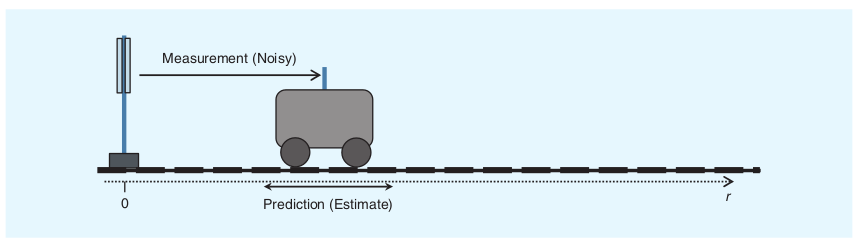
\includegraphics[width=100mm]{images/train0.png}
  \end{figure}
  \item Let state vector \(x_t\) be position and velocity of the train.
    \[
      X_t = \begin{bmatrix} x_t \\ \dot{x_t} \end{bmatrix}
    \]
  \item Train driver by braking or accelerating applies force \(f_t\) for train of mass m
\end{itemize}
\vskip 1cm
\end{frame}

%%%%%%%%%%%%%%%%%%%%%%%%%%%%%%%%%%%%%%%%%%%%%
%Slide 12
\begin{frame}{..Example of modeling}
\begin{itemize}
  \item The control input \( u_t = \dfrac{f_t}{m} \)
  \item Take an example of a train moving along straight railway line
  \item Force is applied between time instances \textit{t} and \textit{(t-1)}
  \item Using kinematic equations, we can write
  \[ x_t = x_{t-1} + ( \dot{x}_{t-1} \times \Delta t ) +  \dfrac{f_t(\Delta t)^2}{2m}  \]
  \[ \dot{x_t} = \dot{x}_{t-1} + \dfrac{f_t \Delta t}{m} \]

\end{itemize}
\vskip 1cm
\end{frame}
%%%%%%%%%%%%%%%%%%%%%%%%%%%%%%%%%%%%%%%%%%%%%
%Slide 13
\begin{frame}{..Example of modeling}
\begin{itemize}
  \item In matrix form:
  \[
    \begin{bmatrix} x_t \\ \dot{x_t} \end{bmatrix} =
    \begin{bmatrix} 1 & \Delta t \\ 0 & 1 \end{bmatrix}
    \begin{bmatrix} x_{t-1} \\ \dot{x_{t-1}} \end{bmatrix} +
    \begin{bmatrix} \dfrac{(\Delta t)^2}{2} \\ \Delta t \end{bmatrix}
    \dfrac{f_t}{m}
  \]
  \item So, by comparing process state equation, we've
  \[ F_t = \begin{bmatrix} 1 & \Delta t \\ 0 & 1 \end{bmatrix} \]
  and
  \[ B_t =  \begin{bmatrix} \dfrac{(\Delta t)^2}{2} \\ \Delta t \end{bmatrix} \]
\end{itemize}
\vskip 1cm
\end{frame}
%%%%%%%%%%%%%%%%%%%%%%%%%%%%%%%%%%%%%%%%%%%%%
%Slide 14
% Enter kalman
% Scilab example
%%%%%%%%%%%%%%%%%%%%%%%%%%%%%%%%%%%%%%%%%%%%%
% Slide 15
% What we do
\begin{frame}{What we do..}
\begin{itemize}
  \item Outdoor: GPS  | Indoors: ?
  \begin{figure} [ht!]
    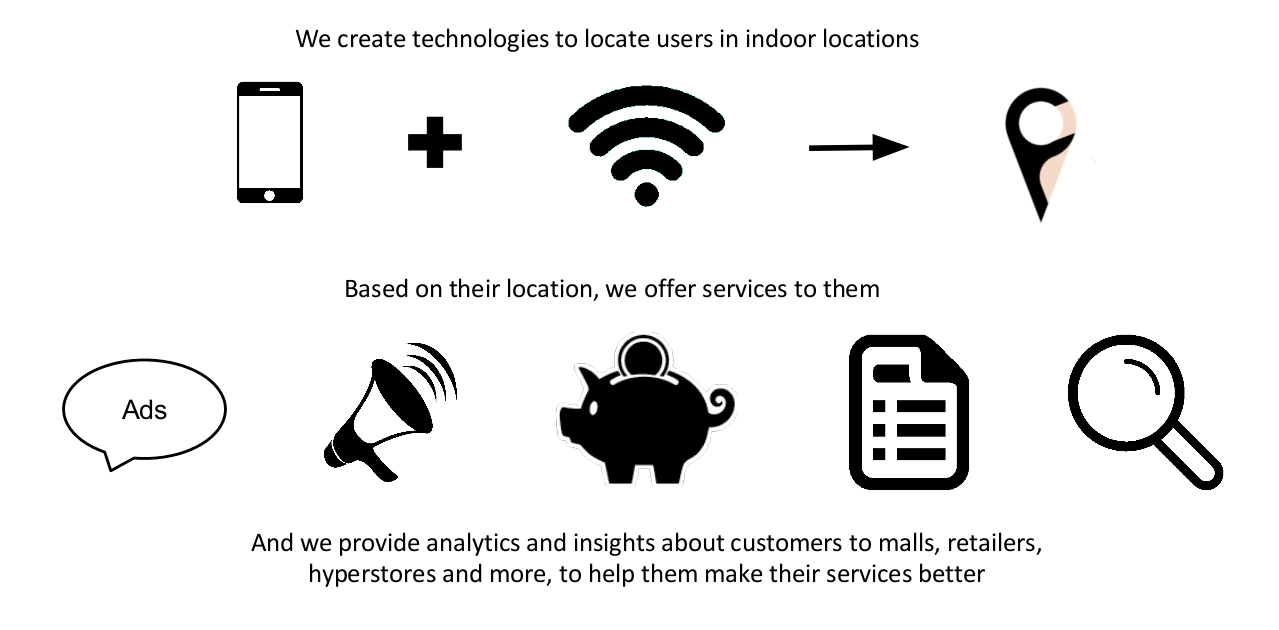
\includegraphics[width=100mm]{images/marketing_pitch.png}
  \end{figure}
  \begin{itemize}
    \item Directly lifted from Marketing pitch deck
    \item I didn't make this
    \item I don't know why there is a magnifying glass
   \end{itemize}
\end{itemize}
\vskip 1cm
\end{frame}
%%%%%%%%%%%%%%%%%%%%%%%%%%%%%%%%%%%%%%%%%%%%%
% Slide 16
\begin{frame}{..What we do}
\begin{itemize}
  \item Basically our system includes:
  \begin{itemize}
    \item A mobile device with WiFi receiver
    \item Public WiFi routers which operate at 2.4/5GHz. At least 3 routers
    \item A human walking on a flat surface
  \end{itemize}
  \item Periodic measurements from WiFi receiver
  \item We don't know where the routers are located inside
  \item We cannot use any additional hardware
  \item We cannot ask the person to inform his/her location at any moment of the time
\end{itemize}
\vskip 1cm
\end{frame}
%%%%%%%%%%%%%%%%%%%%%%%%%%%%%%%%%%%%%%%%%%%%%
% Slide 16
\begin{frame}{..What we do}
\begin{figure} [ht!]
  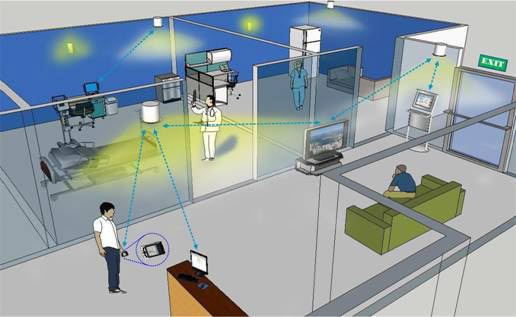
\includegraphics[width=100mm]{images/indoorpositioning.jpg}
\end{figure}
\vskip 1cm
\end{frame}
%%%%%%%%%%%%%%%%%%%%%%%%%%%%%%%%%%%%%%%%%%%%%
% Slide 17
\begin{frame}{..What we do}
\begin{figure} [ht!]
  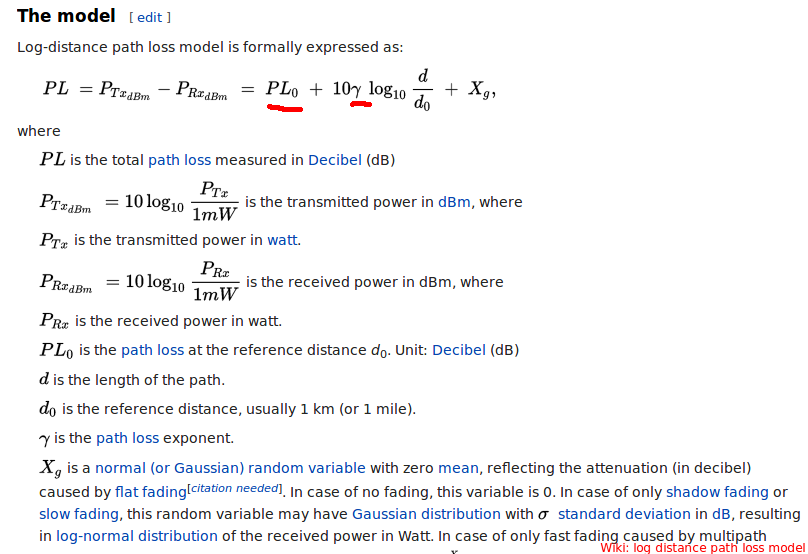
\includegraphics[width=100mm]{images/powerlogmodel.png}
\end{figure}
\begin{itemize}
  \item Strength of WiFi is represented by R.S.S.I. (Received Signal Strength Indication measured in \textbf{dBm})
\end{itemize}
\end{frame}
%%%%%%%%%%%%%%%%%%%%%%%%%%%%%%%%%%%%%%%%%%%%%
% Slide 17
\begin{frame}{..What we do}
\begin{itemize}
  \item Idea is to exploit relationship between RSSI and distance between person and router
  \item Further we go away from router, lesser is measured RSSI
  \item Issue with path loss model: very difficult to ascertain \( PL_0 \) and \(\gamma\)
  \item Hence we resort to a more statistical approach called as WiFi Fingerprinting
  \item Fingerprinting relies recording of the signal strength from several access points in range and storing this information in a database along with the known coordinates
\end{itemize}
\vskip 1cm
\end{frame}


% Problems we face
% How we used kalman filter
% What is FKF
% Results
% Problems using Kalman filter
% Summary

%%%%%%%%%%%%%%%%%%%%%%%%%%%%%%%%%%%%%%%%%%%%
% Slide 10
\begin{frame}{References/Links}

\begin{itemize}
  \item Source code \url{https://github.com/gnu-sandhi/sandhi.git}
  \item Documentation \url{https://github.com/gnu-sandhi/docs.git}
  \item Problems using it? Found a bug?
  \begin{itemize}
 	\item Are you sure its a bug and \textbf{not} \textit{a feature}?
	\item Raise an issue on our github
	\item Mailing List: \textit{gnu\_lc@googlegroups.com}
  \end{itemize}
\end{itemize}

\vskip 1cm

\end{frame}
%%%%%%%%%%%%%%%%%%%%%%%%%%%%%%%%%%%%%%%%%%%%%

\end{document}
